\documentclass[12pt]{article}
\usepackage{amsmath}
\usepackage{graphicx}
\usepackage{subfigure}
\usepackage{listings}

\usepackage[margin=1in]{geometry}
\lstset{
breaklines=true
}

\DeclareFixedFont{\ttb}{T1}{txtt}{bx}{n}{12} % for bold
\DeclareFixedFont{\ttm}{T1}{txtt}{m}{n}{12}  % for normal

% Custom colors
\usepackage{color}
\definecolor{deepblue}{rgb}{0,0,0.5}
\definecolor{deepred}{rgb}{0.6,0,0}
\definecolor{deepgreen}{rgb}{0,0.5,0}

\usepackage{listings}

% Python style for highlighting
\newcommand\pythonstyle{\lstset{
language=Python,
basicstyle=\ttm,
otherkeywords={self},             % Add keywords here
keywordstyle=\ttb\color{deepblue},
emph={MyClass,__init__},          % Custom highlighting
emphstyle=\ttb\color{deepred},    % Custom highlighting style
stringstyle=\color{deepgreen},
showstringspaces=false            % 
}}


% Python environment
\lstnewenvironment{python}[1][]
{
\pythonstyle
\lstset{#1}
}
{}

\begin{document}

\title{In-Class Kaggle Competition Writeup}
\author{Hanqiu Xia}

\maketitle

\section{Exploratory Analysis}
The dataset I use for this competition is about Allstate claims severity and it contains 132 columns.  The first column represents the ID for each observation and  I remove this column in later analysis, while the last column records the loss of insurance in US dollar,  which is the target variable in my analysis. The middle 130 variables are all independent variables, including 116 categorical variables and 14 numerical variables. I apply different visualization  techniques on distinct types of variables in order to get an idea of how to pre-process these variables and what model might work for them.  \\

 I draw count plot for each categorical features.  Based on the plots, we know that cat1 to cat72 have only two labels, A and B. For most cases, label A has the majority entries, which means these variable lesslikely provide much information in predicting result, so we may consider to drop them off. Cat73 to cat80 have three or four labels, and Cat81to cat116 have more than 5 labels.\\

For numerical variables, I first plot the distribution graph. I notice that most of variables have multiple peaks, and some of them are obviously skewed, therefore, I think normalization is necessary before we fit the model.\\

I also calculate the correlation between every pair of numerical variables with considering the potential high collinearity issue. The collinearity problem has more influence on linear model than non-linear model. I  just search for pair of attributes that with correlation higher than 0.7 and find out the highest correlation contributed by cont11 and cont12. Their correlation is 0.99, which means they are almost perfect linear, so we must remove one of them. Cont1 and cont 9 are also highly correlated, hence, it is safe to remove one of them.  In addition, I graph scatter plot for high correlated  pair of variables to visualise and evidence their correlations.\\

Moreover, I plot the histogram for dependent variable loss, and find that it is highly skewed. Hence, I take log on it, which make it becomes nearly normal.



\section{Models}

I choose two models to generate prediction -- Lasso regression and extreme gradient boosting model.\\  

Lasso regression is a simple linear model with only one regularisation parameter.  The penalty of Lasso is the sum of absolute value of the coefficients, therefore, it would automatically shrink coefficients of those insignificant and collinear variables towards zero in order to minimize the penalty. However, other linear models, like Ridge with penalty as the sum of the squares of coefficients,  cannot do the parameter shrinkage or variable selection. I use \texttt{LassoCV} from package \texttt{sklearn.linear$\_$model} to implement lasso regression and hyperparame selection simultaneously.\\

Extreme gradient boosting, also known as the xgboost, is a nonlinear model created by Tianqi Chen.  Just as its name suggested, xgboost is the limit of implementation of gradient boosting. Xgboost  has faster execution speed than other implementation of gradient boosting and bagged decision tree. In addition, xgboost has excellent performance  on classification and regression predictive modeling problems. I apply \texttt{XGBRegressor}  from package \texttt{xgboost} to implement xgboost.

\section{Training}

Lasso regression is trained with L1 prior as regularizer, and the optimization objective for Lasso is:

$$\min_{\lambda} \dfrac{1}{n}\sum_{i} (y_i-\lambda^Tx_i)^2+C||\lambda||.$$

Lasso is aimed to find the coefficients for attributes that contribute to a small mean square error and a small regularization simultaneously. However, there is a  trade-off between loss function and regularization term. We may need include many variables in our model to gain smaller loss, but the regularization term will definitely  increase and likely result in an overfitting issue. Therefore, in this case, hyperparameter selection is necessary, and I will explain this in detail in next section. Lasso regression takes about 11s in this numerical experiment.\\


The xgboost model implements the gradient boosting decision tree algorithm. Gradient boosting is an ensemble technique where new models are added to correct the errors made by existing models. Models are added sequentially until no further improvements can be made.  During the boosting algorithm, we are aimed to find the weight on different models and apply a gradient descent algorithm to minimize the exponential loss when adding new models. The  simple xgboost model without any hyperparameter selection takes about 44s, while a compex xgboost with hyperparameter tuning takes 5 hours!


\section{Hyperparameter Selection}

Lasso regression has only one hyperparameter, which is the regularization parameter $C$ in the regularization term.  In order to tune this hyperparameter and achieve some degree o optimality, I select a list of potential hyperparameters and try to see which one performs the best. I implement \texttt{LassoCV} to fulfill this idea, this function fits model on grid of $C$ and estimates the best $C$ by cross validation. The following  graph shows the functional relation between predictive accuracy on some subset of the training data and a varying hyperparameter. \\

 \begin{figure}[htbp]
\begin{center}
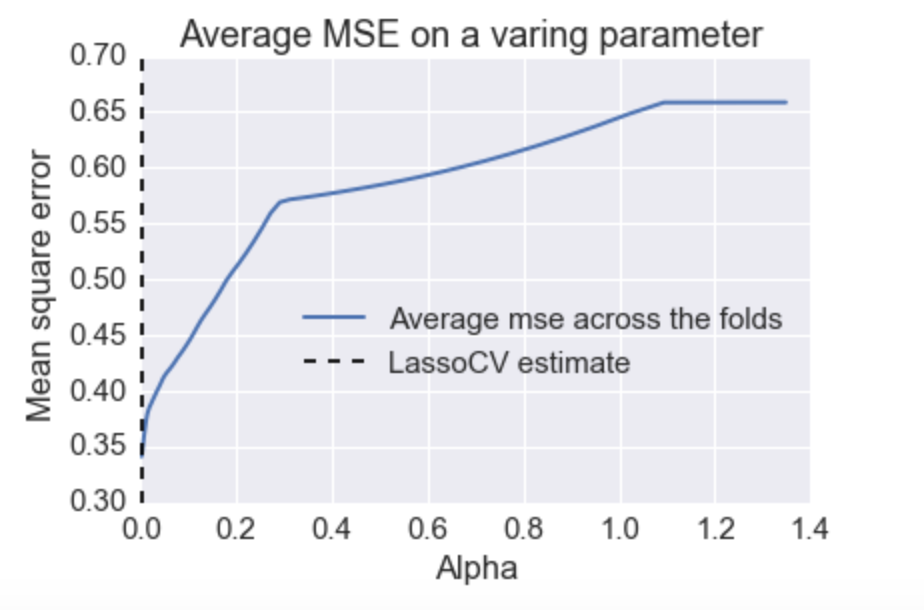
\includegraphics[width=3.5in]{lasso1.png}
\caption{Average mean square error aross folds on a varing hyperparameter}
\end{center}
\end{figure}


In the above figure, the best regularization parameter with high predictive accuracy is close to 0. \\

Xgboost model has several hyperparameters, inlcuding the number of boosted trees to fit, the maximum tree depth and etc. Similarly, for each hyperparameter, I have a list of choices, and the ultimate goal is to find the best model among all combinations of these hyperparameters. I apply \texttt{GridSearchCV} to fulfill this goal. In this function, the hyperparameters in the model are optimized by cross-validated grid-search over a parameter grid.  According to the results, the best value for maximum tree depth, the number of boosted tree and minimum child weight is 6, 100 and 3, respectively.  These values are just the best ones among the choices of parameters I list and they are not the global optimal for the model.

\section{Data Splits}

In order to avoid the overfitting issue, I implement cross validation on both models. The idea of $K$-fold cross validation is to divide the dataset into $K$ folds. Train the algorithm on $K-1$ folds and compute the evaluation measure on the last fold. Then, repeat this $K$ times, using each fold in turn as the test fold. Next, compute the mean of the evaluation measure over the $K$ folds. The function scheme will implement this process on every choice of hyperparameter or every combination of hyperparameters and finally choose one with the best mean of evaluation measure. 



\section{Errors and Mistakes}

The xgboost algorithm is really slow when I use grid search cross validation to tune the hyperparameters.  I think it is because the parameter pool I provides is large, it contains several hyperparameters that needed to be tuned and  each hyperparameter includes several candidates. Moreover, I also implement the K-fold cross validation for each iteration in order to avoid the overfitting issue which further slack computational speed.  I think the hardest part of this competition is fine tuning, since I do not have the prior information about which hyperparameters are more needed to be tuned than others, and I don't know the common range of these hyperparameters, either. Thus, it would take  me  long time to find an optimal model.



\section{Predictive Accuracy}
I have uploaded the result of the my best model -- xgboost  to Kaggle, and my username for Kaggle is Hanqiu.\\

To test the effectiveness of these two models, I train models on some subset of training dataset and evaluate them on the rest of training dataset by calculating the mean-absolute-error. To be specific, I take $80\%$ of original training dataset as the new training dataset, and take the rest of $20\%$  as the new test dataset. The mean-absolute-error for lasso regression is 1328.70, while it is 1160.89 for xgboost model.  The following graph could also evidence the exceptional perform of xgbboost over lasso. 

\begin{figure}[htbp]
\begin{center}
\hspace*{-40pt}
\begin{tabular}{c}
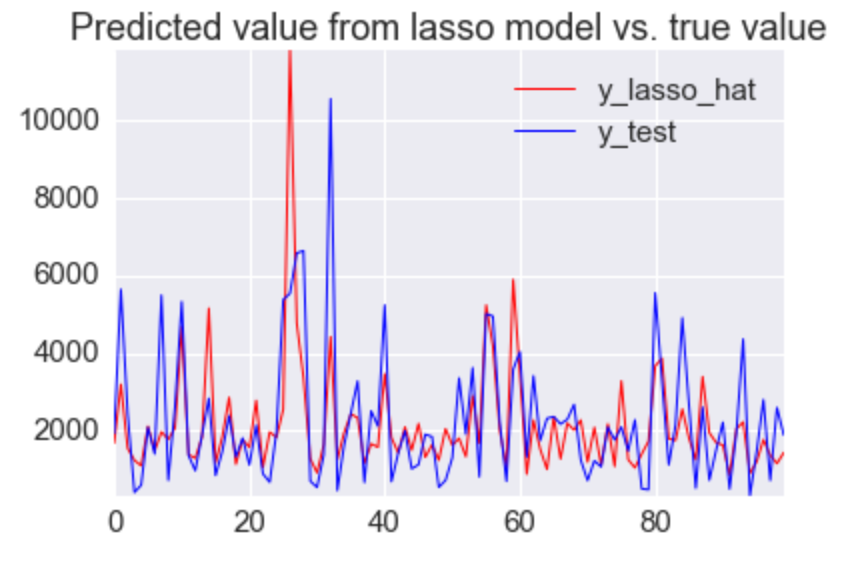
\includegraphics[width=3.3in]{testlasso.png} 
\hspace*{-20pt}
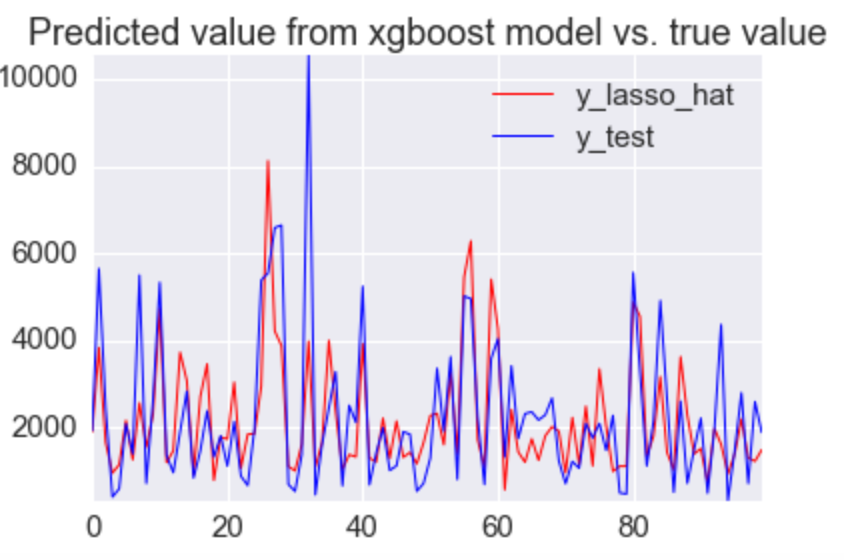
\includegraphics[width=3.3in]{testxgb.png}
\end{tabular}
\end{center}
\caption{Left: The first 100 points from predicted value of lass model vs. the first 100 points in true test values; Right: The first 100 points from predicted value of xgboost model vs. the first 100 points in true test values}
\label{fig: sobol}
\end{figure}

For better visualization, I just choose to show the first 100 predicted values and true values. We can see from the figure 2 that predicted values from xgboost follows the true values better than those from lasso.

\section{Code}

\begin{python}
import numpy as np
import pandas as pd
import matplotlib.pyplot as plt
%matplotlib inline
from sklearn.linear_model import Lasso
from sklearn.linear_model import Ridge
from sklearn.model_selection import KFold
import seaborn as sns
import random
import xgboost as xgb
from xgboost import XGBRegressor
from sklearn.ensemble import RandomForestRegressor
import warnings
warnings.filterwarnings("ignore")
from sklearn.grid_search import GridSearchCV
import time

# Load data
data_train = pd.read_csv("/Users/apple/Desktop/duke/Fall2016/CS571/HW5/pml_train.csv")
data_test = pd.read_csv("/Users/apple/Desktop/duke/Fall2016/CS571/HW5/pml_test_features.csv")
# Remove the first column
data_train = data_train.ix[:,1:len(data_train.columns)]

# Find the columns with categorical data in training dataset and change them to 0/1
cols = data_train.columns
num_cols = data_train._get_numeric_data().columns
cat_col = list(set(cols) - set(num_cols))
for column in cat_col:
    data_train[column] = pd.factorize(data_train[column].values, sort=True)[0]
# Find the columns with categorical data in test dataset and change them to 0/1
cols_test = data_test.columns
num_cols_test = data_test._get_numeric_data().columns
cat_col_test = list(set(cols) - set(num_cols))
for column in cat_col_test:
    data_test[column] = pd.factorize(data_test[column].values, sort=True)[0]

# Plot the bar plot on every categorical features
n_cols = 6
n_rows = 20
for i in range(n_rows):
    fg,ax = plt.subplots(nrows=1,ncols=n_cols,sharey=True,figsize=(12, 3))
    for j in range(n_cols):
        sns.countplot(data_train.ix[:,i*n_cols+j],ax=ax[j])
# Get the dataframe with numerical data
data_train_num = data_train[num_cols]
data_train_num = data_train_num.ix[:,:-1]
# Get the distribution plot for each numerical variable
n_cols = 7
n_rows = 2
for i in range(n_rows):
    fg,ax = plt.subplots(nrows=1,ncols=n_cols,sharey=True,figsize=(12, 2))
    for j in range(n_cols):
        sns.distplot(data_train_num.ix[:,i*n_cols+j],ax=ax[j])
# Calculates  coefficient for all combinations
data_corr = data_train_num.corr()

corr_pair= []
threshold = 0.7

#List pairs that are highly correlated, say greater than threshold
for i in range(len(data_corr.columns)): 
    for j in range(i+1,len(data_corr.columns)): 
        if (np.abs(data_corr.ix[i,j]) >= threshold and np.abs(data_corr.ix[i,j]) < 1):
            corr_pair.append([data_corr.ix[i,j],i,j]) 

#Sort pair from highest to lowest           
corr_pair_s = sorted(corr_pair,reverse=True)

#Print correlations and column names
for c,i,j in corr_pair_s:
    print ("%s and %s = %.2f" % (cols[i],cols[j],c))

# Plot scatter plot on each selected pair of features
n_cols = 5
n_rows = 3
fg,ax = plt.subplots(3,5,figsize=(12, 8))
for i in range(n_rows): 
    for j in range(n_cols):
        ans = corr_pair_s[i*n_cols+j]
        ax[i,j].plot(data_train_num.ix[:,ans[1]],data_train_num.ix[:,ans[2]],".",)
for axs in ax.ravel():
    axs.margins(0.05)
pass

# Split traing dataset into X and y
data_train_x = data_train.ix[:,:-1]
data_train_y = data_train.ix[:,-1]
data_test_x = data_test.ix[:,1:]

# Visualize the distribution plot of y 
sns.distplot(data_train_y)
# Since the distribution plot of y is highly skewed, it's better to take log on it and get a normal distribution 
data_train_y_log = np.log(data_train_y)
sns.distplot(data_train_y_log)
plt.show

# lasso cv
from sklearn.linear_model import LassoCV
import time

#record the runtime
start_time = time.time()
lcv = LassoCV(cv=10,normalize = True).fit(data_train_x,data_train_y_log)
time_lcv = time.time() - start_time

# Calculate the average mse aross the fold for every choice of alpha
mse = np.mean(lcv.mse_path_,axis= 1)


plt.plot(lcv.alphas_,mse,label='Average mse across the folds', linewidth=2)
plt.axvline(lcv.alpha_, linestyle='--', color='k',label='LassoCV estimate')
plt.legend(loc='bottom right', bbox_to_anchor=(1, 0.5))
plt.xlabel('Alpha')
plt.ylabel('Mean square error ')
plt.title("Average MSE on a varing parameter ")
plt.axis('tight')
print("runtime for lasso_cv is ",time_lcv,"s")

# Save the result
y_lcv = np.exp(lcv.predict(data_test_x))
result_lcv = pd.DataFrame()
result_lcv['id'] = data_test.id
result_lcv['loss'] = y_lcv

result_lcv.to_csv('result_lasso.csv', index=False)

# First,fit a simple xgboost without any hyperparameter selection
start_time = time.time()
xgb = XGBRegressor()
xgb.fit(data_train_x,data_train_y_log)

time_xgb = time.time() - start_time
print("Runtime for simple xgb is", time_xgb, "s")

# Hyperparameter selection
start_time = time.time()
xgb = XGBRegressor()
param_grid = { 
     'n_estimators': [10, 50, 100],
     'min_child_weight': [3,5,7],
     'max_depth': [5,10,15,20]
}

# Grid search cv for xgb
CV_xgb = GridSearchCV(estimator=xgb, param_grid=param_grid, cv = 5)

# Fit the best model among the parameters combination in the parameter pool 
CV_xgb.fit(data_train_x, data_train_y_log)

time_xgbcv = time.time() - start_time
print("Runtime for xgb with hyperparameters selection is", time_xgbcv, "s")

# Get the best parameters
CV_xgb.best_params_

# predicted values
y_hat = np.exp(CV_xgb.predict(data_test_x))
# save the result
result_xgb = pd.DataFrame()
result_xgb['id'] = data_test.id
result_xgb['loss'] = y_hat

result.to_csv('result_xgb.csv', index=False)


from sklearn.cross_validation import train_test_split


# Split the original trainig dataset into new training dataset and test dataset
train, test= train_test_split(data_train, test_size=0.20, random_state=42)
train_x = train.ix[:,:-1]
test_x = test.ix[:,:-1]
train_y = train.ix[:,-1]
test_y = test.ix[:,-1]
train_y_log = np.log(train_y)
# Evaluate the effectiveness of lasso and xgboost via mean absolute error
# lasso
lcv_test = LassoCV(cv=10).fit(train_x,train_y_log)
y_lcv_hat = np.exp(lcv_test.predict(test_x))
# xgboost
xgb_test = XGBRegressor(max_depth=6,min_child_weight = 3,n_estimators= 200)
xgb_test.fit(train_x,train_y_log)
# predicted value
y_xgb_hat = np.exp(xgb_test.predict(test_x))
from sklearn.metrics import mean_absolute_error

# compute the mean-absolute-error for two models
abe_lasso = mean_absolute_error(y_lcv_hat, test_y)
abe_xgb = mean_absolute_error(y_xgb_hat, test_y)
print ("The mean absolute error for Lasso is", abe_lasso)
print ("The mean absolute error for xgb is", abe_xgb)
# visually represent the accuracy of my models and the predictions 
plt.plot(range(100),y_lcv_hat[0:100],'r-',linewidth = 1, label = "y_lasso_hat")
plt.plot(range(100),test_y[0:100],'b-',linewidth = 1,label = "y_test")
plt.title('Predicted value from lasso model vs. true value')
plt.axis('tight')
plt.legend()

plt.plot(range(100),y_xgb_hat[0:100],'r-',linewidth = 1,label = "y_lasso_hat")
plt.plot(range(100),test_y[0:100],'b-',linewidth = 1,label = "y_test")
plt.title('Predicted value from xgboost model vs. true value')
plt.axis('tight')
plt.legend()


\end{python}


\end{document}